%% entwurf.tex
%% $Id: entwurf.tex 28 2007-01-18 16:31:32Z bless $
%%
%% ==============================
\chapter{Design}
\label{ch:Design}
This master thesis aims to compare different positions on the ear for body temperature measurement. 
To achieve this, a prototype was developed in this master thesis, which allows temperature measurements at different positions in and around the ear. 
Subsequently, studies were conducted to collect temperature data at different locations in and around the ear and analyze the collected data.
At the beginning of this section, the OpenEarable platform is described. This is the basis of the prototype and forms the basis for understanding. Then, the sensors are explained, since they are essential for the temperature measurement.
After laying the groundwork for understanding the prototype, the development and approach to designing the prototype is described.
In addition, the detailed methodology and procedure of the study are described.
The study results are not described here, all details are described in the \ref{ch:Evaluation} chapter.

\section{Platform: OpenEarable}
\label{ch:Design:Prototype:OpenEarable}

In Chapter \ref{Background:SensingWithEarables:OpenEarable}, the OpenEarable platform is thoroughly described, emphasizing its interaction with other components. 
The OpenEarable was designed for rapid prototyping and exploration of novel Earable applications, and this thesis successfully utilized it as the foundation for the prototype. 
Figure \ref{fig:design:prototype_connection} illustrates the seamless collaboration between all components. 
Leveraging an Arduino Nano 33 BLE, the OpenEarable enables the deployment of Arduino-based software, and its connection to both the PCB and FlexPCB is facilitated via the 4-pin connector. 
The developed software gathers data from the temperature sensors and effectively utilizes the OpenEarable's resources. 
The study data is persistently stored on the SD card, and the study termination is triggered by a double-click on the push button.
In summary, the OpenEarable platform proved to be a versatile and effective foundation for the prototype, enabling seamless interaction between its components and facilitating data collection from the temperature sensors. 
By leveraging Arduino-based features and user-friendly design, OpenEarable was successfully used in this study to explore novel Earable applications and conduct the user study easily and efficiently.

% TODO: PCB Schematic in den Anhang vermutlich packen, sehr wichtig!!!

\section{Sensors}
\label{ch:Design:Prototype:Sensors}

Based on research and experience at the TECO Institute, the MLX90632 sensor was selected for its suitability for our project.

The MLX90632 sensor is an infrared temperature sensor known for its high accuracy in temperature measurements. This enables reliable applications where precise temperature tracking is needed.
Furthermore, non-contact temperature measurement is a huge advantage. 
The MLX90632 can measure temperature without physical contact with the object or body part, providing a non-invasive and convenient ear temperature monitoring option.
In order to place the temperature sensors in the necessary locations to measure temperature, the sensors must be appropriately small. 
Since the MLX90632 has a small form factor, this is optimal for the application needed.
Additionally, the MLX90632 is readily available on the market and has existing Arduino libraries. 
This availability and compatibility with Arduino simplify the integration process and save valuable development time.
In addition, the sensor is designed for low power consumption, making it suitable for battery-powered devices. 
Given the small battery size in the developed prototype, low power consumption is critical for extended operation during the study.
The MLX90632 offers fast response times and allows for real-time temperature monitoring and fast updates. 
Some difficulties arose when writing the EEPROM, so the default value was left at 2Hz.
The intention of adjusting the measuring rate was the implementation details of the library, which was finally solved by adjusting the library. 
This process is described in more detail in the chapter \ref{TODO: ann ref}.
The high sensitivity to temperature changes allows the MLX90632 to accurately detect even minor variations. This sensitivity is advantageous for precise temperature tracking.
In addition, the sensor has applications in both the consumer and industrial markets due to its accuracy and reliability. This versatility makes it an excellent choice for our master's thesis project, which involves working with an Arduino Nano 33 BLE.

The MLX90632 has 4 pins that must be connected. Beside 3.3V and Ground the MLX90632 has a SCL and SDA connector. SCL stands for the clock signal, and SDA for the data flow.

Overall, infrared temperature sensing capabilities, accuracy, easy availability, non-invasive measurement, compact size, and compatibility with Arduino make the MLX90632 an ideal choice for the developing ear temperature monitoring system.


\section{Prototype}
\label{ch:Design:Prototype}
To measure the temperature as planned in Section \ref{ch:Introduction:PlannedApproach}, a custom-built prototype was developed as part of this master thesis.
The prototype consists of two components: an earpiece that resembles an in-ear headphone and a component placed behind the ear that resembles a hearing aid. TECO's OpenEarable platform for ear-based observations is integrated into the behind-the-ear component. This component serves as the central interface and houses the Arduino on which all code is executed. Additionally, a circuit board with three temperature sensors is connected to measure the temperature behind the ear.
The second component is placed in the ear and is also controlled by the OpenEarable via the Arduino Nano33 BLE installed there. The OpenEarable acts as the basis for reading and storing data from the sensors connected via I2C. The relationship and interaction of the components are visually represented in Figure \ref{fig:design:prototype_connection}.
To ensure functionality and protection of the hardware, custom 3D-printed enclosures were created for both the behind-the-ear component and the in-the-ear component. 
Figure \ref{fig:design:prototype_on_head_visual} shows the final result, worn by a participant, and also visually demonstrates the positioning of the components.
As shown in \ref{fig:design:prototype_on_head_visual}, the custom cases add durability and a high-end appearance to the product, improving its overall usability and aesthetics.
The use of the 8-pin cable effectively connects the two components, additionally ensuring good comfort.

\begin{figure}[t]
    \centering
    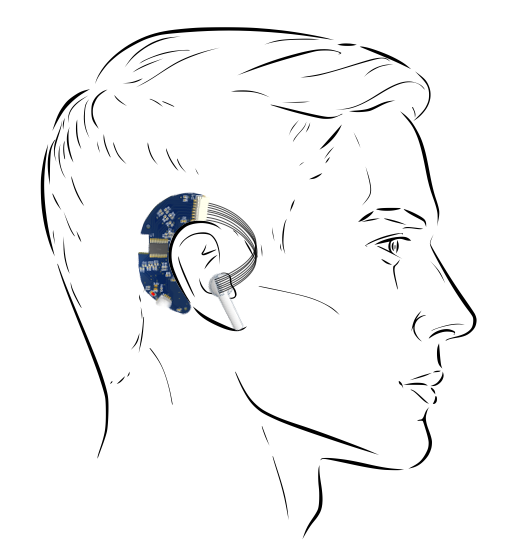
\includegraphics[width=0.48\textwidth]{thesis-doc/images/prototype/prototype_on_head_visual.png}
    % TODO: the second picture should be replaced with an original photo
    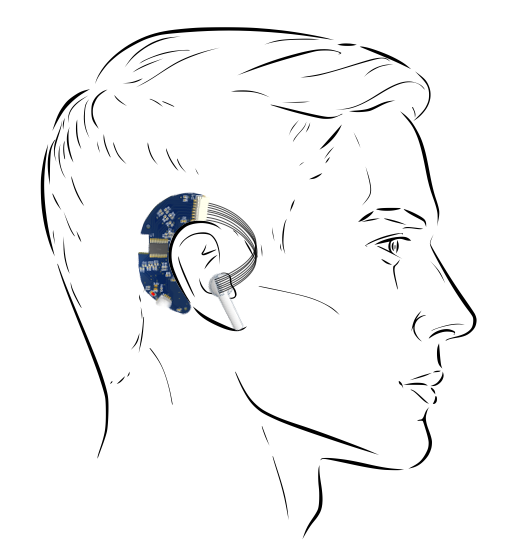
\includegraphics[width=0.48\textwidth]{thesis-doc/images/prototype/prototype_on_head_visual.png}
    \caption{Visual view when theoretically carrying the components without wrapping the component behind the ear. The PCB behind the ear measures in 3 positions (bottom, middle, top) and is connected to the FlexPCB via an 8-pin connector, which is visually already wrapped in the sleeve here. The wiring of the two components results in good stability when worn, so the device cannot fall off. In addition to this visual representation, the prototype can be seen in a real environment including the cases.}
    \label{fig:design:prototype_on_head_visual}
\end{figure}

\begin{figure}
    \centering
    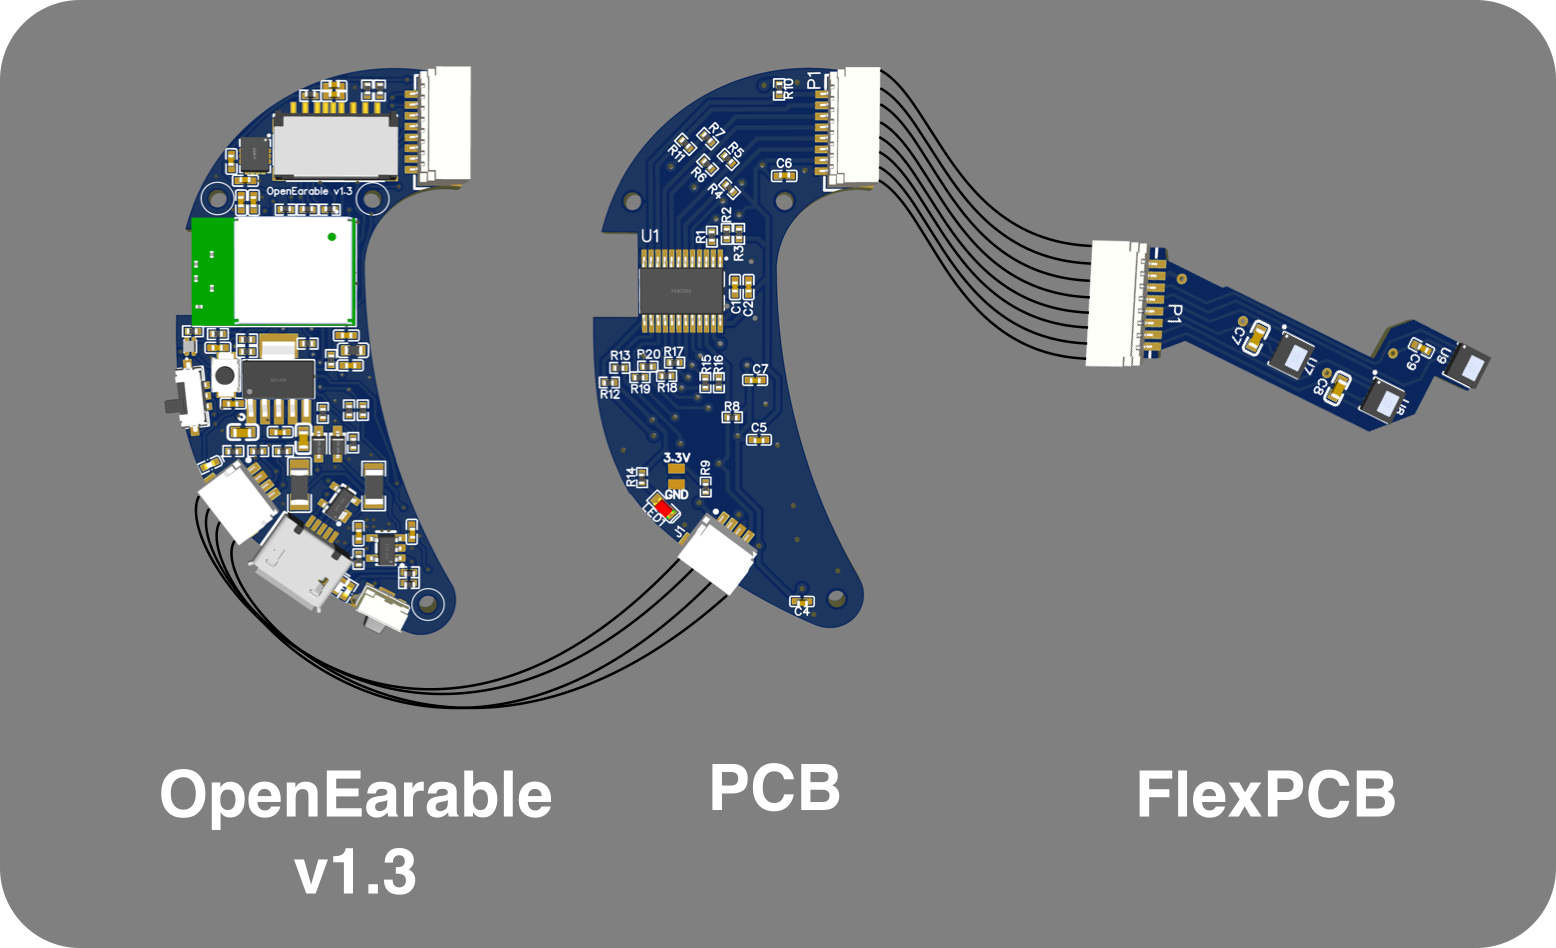
\includegraphics[width=\textwidth]{thesis-doc/images/prototype/PrototypeConnection.png}
    \caption{Visual representation of the prototype and the interaction of all components. The PCB is connected to the OpenEarable v1.3 with a 4-pin connector. In the OpenEarable is an Arduino Nano33 BLE, with which it is possible to control the multiplexer (TCA9548A) via I2C. Through this, every sensor value on the PCB and also on the FlexPCB can be read out, since the FlexPCB is also connected to the multiplexer via the 8-pin connector.}
    \label{fig:design:prototype_connection}
\end{figure}

\begin{figure}
    \centering
    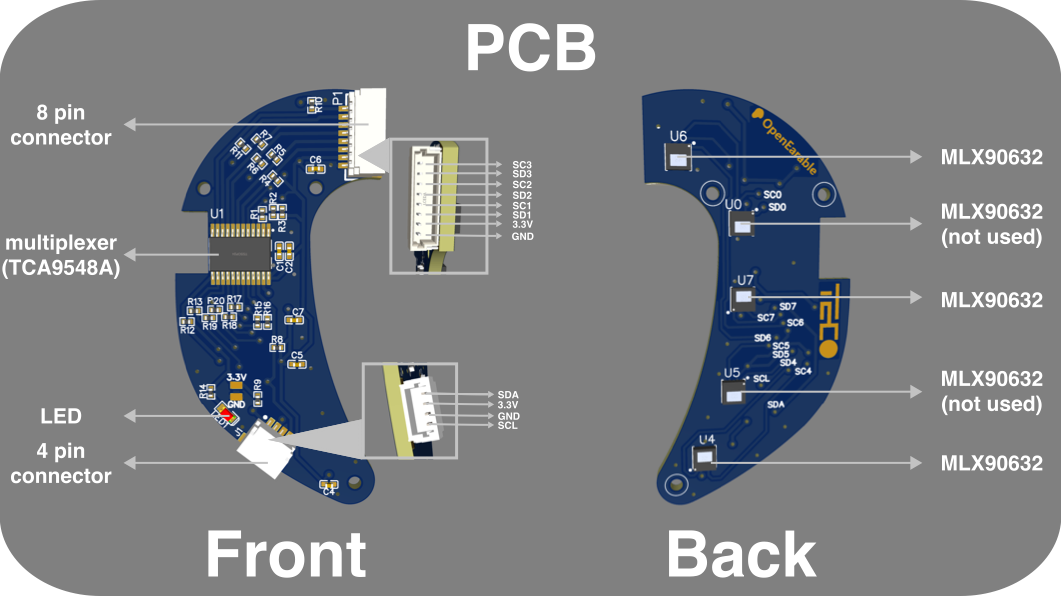
\includegraphics[width=\textwidth]{thesis-doc/images/prototype/PCB_Description.png}
    \caption{Representation of the front and back of the PCB. The multiplexer can be seen on the front, which is controlled by the OpenEarable via the 4-pin connector. The three other MLX90632 are then connected by the FlexPCB via the 8-pin connector. In addition, an LED is connected to the front, which lights up green if no short circuit is generated. The temperature sensors can be seen on the back, but only three of the five connections visible in the design are used.}
    \label{fig:design:pcb_description}
\end{figure}

\subsection{Temperature Measurements Behind the Ear}
\label{ch:Design:Prototype:BehindEar}

The temperature behind the ear is measured at 3 positions, as can be seen in Figure \ref{fig:design:pcb_description} on the back of the PCB.
To position the temperature sensors at the locations chosen in section \ref{ch:Introduction:PlannedApproach}, a PCB was developed that has the sensors installed at the appropriate locations. 
The PCB has been designed so that only the temperature sensors are placed on the back. This allows the PCB to be placed entirely in the bottom of the case, while the temperature sensors peek out through matching openings in the case. On the front of the PCB are all the other components, including a 4-pin connector and an 8-pin connector.
The 4-pin connector is used to connect to the OpenEarable. This connection allows the OpenEarable to communicate with the PCB via I2C, as the OpenEarable also has a special 4-pin connector for this purpose.
To be able to control the second component (the earpiece) via I2C later on as well, the 8-pin connector was added to establish a connection to the second component.
Via I2C, the built-in multiplexer is addressed, with which one of the eight possible applied lines can be switched and read out. The eight possible through-connections of the multiplexer are connected to all temperature sensors, including those of the FlexPCB via the 8-pin connector.
In addition, an LED is installed on the PCB to directly indicate a possible short circuit.
For each temperature sensor, the signals Ground, Power (3.3V) as well as SCL (clock signal) and SDA (data transmission) are required, as shown in Figure \ref{fig:design:pcb_description}. Communication with the multiplexer can be handled through the 4-pin connector.
To connect the 3 temperature sensors of the FlexPCB, a total of 12 signals are required, which can be reduced somewhat. For this purpose, the ground and power signals can be used together, resulting in a total of 8 signals being transmitted.

A case has now been developed around the OpenEarable and the custom-made PCB to enable a comfortable fit.
Above the PCB, the battery is placed in the enclosure so that no long cables are needed for the power supply to record the data in the study conducted.
The OpenEarable is placed above this.
The dimensions of the PCB are exactly the same as the OpenEarable to keep the case as small and compact as possible.
The sensor used requires an angle of $ 50 ^ \circ$ around itself for the temperature to be reliably measured. 
This was taken into account.
The layered representation for visualization can be seen in Figure \ref{fig:design:prototype_behind_head_layered_view}.

\begin{figure}
    \centering
    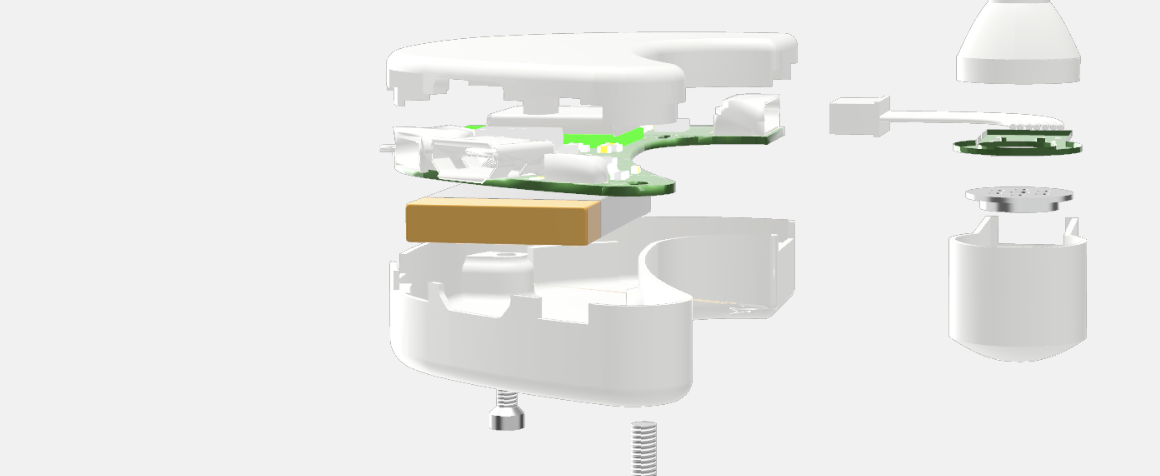
\includegraphics[width=\textwidth]{thesis-doc/images/prototype/Prototype_PCB_layered_view.png}
    \caption{Layered view of the component behind the ear. At the bottom is the designed PCB as the temperature sensors can look out towards the skin. The battery is placed between the PCB and the OpenEarable.}
    \label{fig:design:prototype_behind_head_layered_view}
\end{figure}

\subsection{Temperature Measurements in the Ear}
\label{ch:Design:Prototype:Earpiece}

The second component now enables temperature measurement in the ear area. The FlexPCB itself is only equipped with components on the front side. Thereby, the 8-pin connector that connects the FlexPCB to the PCB is located, as described in section \ref{ch:Design:Prototype:BehindEar}. Additionally, three temperature sensors are placed on the FlexPCB to sense the positions in the ear and pinna described in section \ref{ch:Introduction:PlannedApproach} and Figure \ref{fig:ear_measurement_positions}.
The FlexPCB was designed to extend through the component. On the one hand, the 8-pin connector protrudes outward to connect to the PCB. On the other hand, the PCB runs along the outside of the housing to the earbud, allowing the FlexPCB to snake through. The tip of the FlexPCB also contains a temperature sensor mounted in the earplug and aimed directly at the eardrum. Another temperature sensor is aimed at the ear canal and is located on the outer edge of the earplug. The third temperature sensor is aimed at the pinna.
The component was modeled on the design of an AirPod, but heavily modified afterward. The original AirPods design is freely available on TinkerCAD and was used as the basis for the component shape. The inside of the design was completely hollowed out to allow cables to be routed through the case. Additionally, an adapter was added to the side to fit the redesigned earpod. An earbud can be attached here to ensure that the earbud penetrates further into the ear than usual compared to conventional in-ear headphones. This enables precise temperature measurement in the direction of the eardrum. A temperature sensor is attached to the tip of the earbud to perform basic temperature measurements.
The three temperature sensors on the FlexPCB can be switched via the multiplexer that is connected to the PCB. This allows for precise selection and acquisition of the desired measurements. Figure \ref{fig:design:prototype_earpiece_views} shows a sketch and other images of the final component.

\begin{figure}[!h]
    \centering
    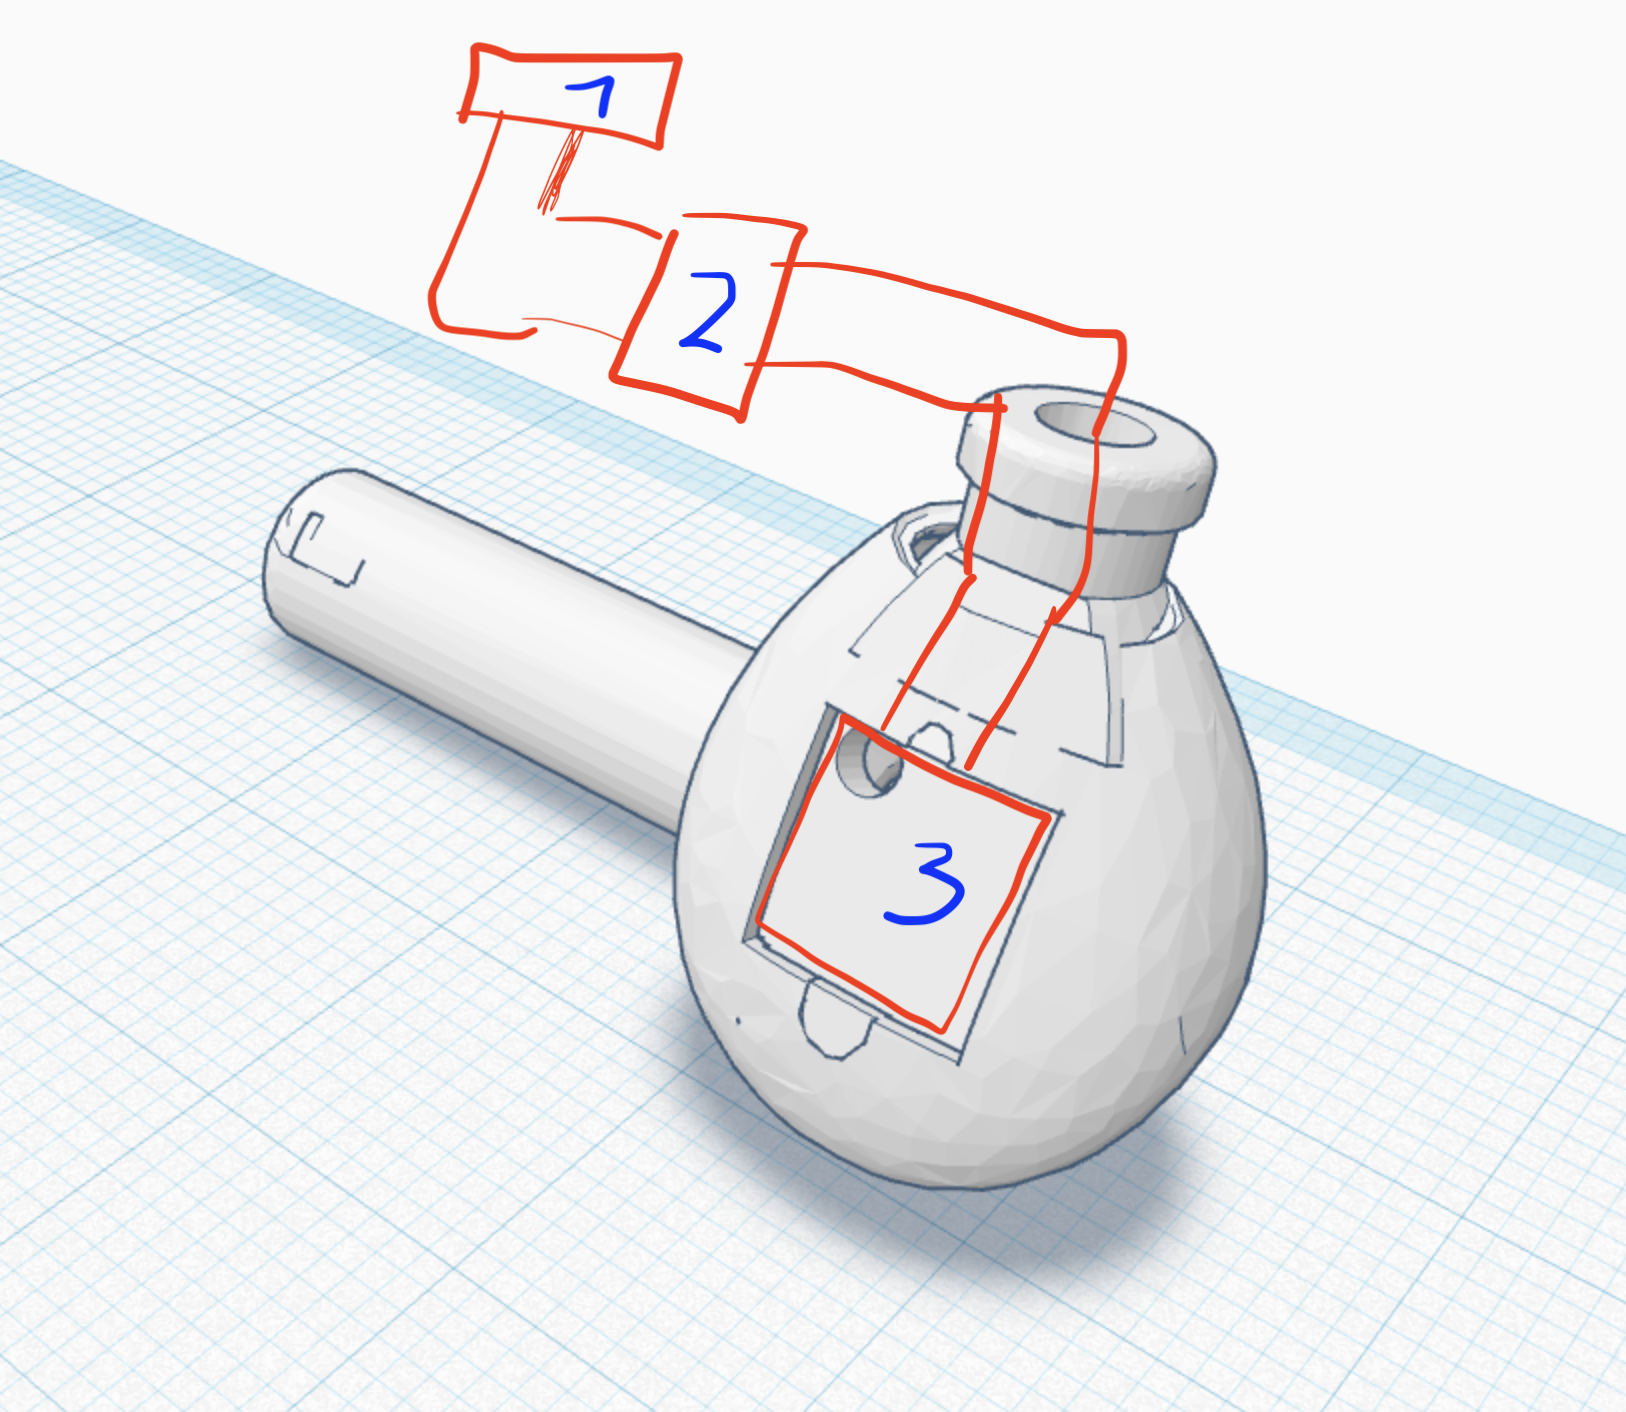
\includegraphics[width=0.48\textwidth]{thesis-doc/images/prototype/flex_pcb_design_finding.png}
    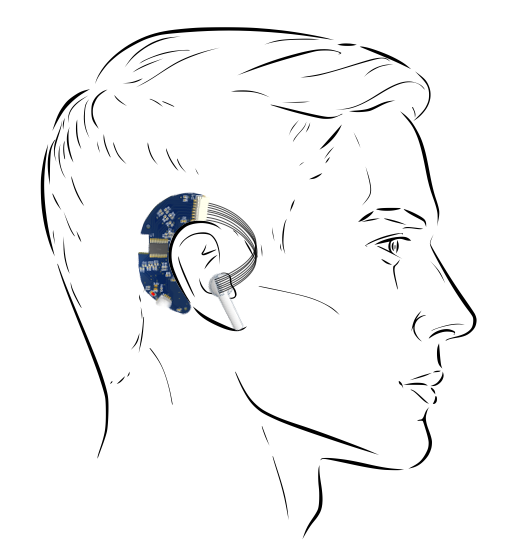
\includegraphics[width=0.48\textwidth]{thesis-doc/images/prototype/prototype_on_head_visual.png}
    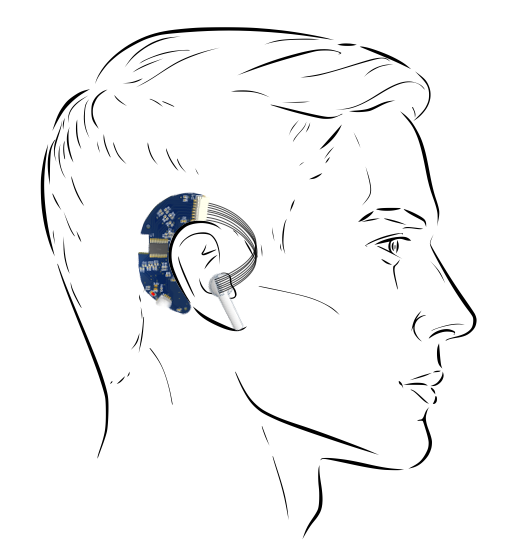
\includegraphics[width=0.48\textwidth]{thesis-doc/images/prototype/prototype_on_head_visual.png}
    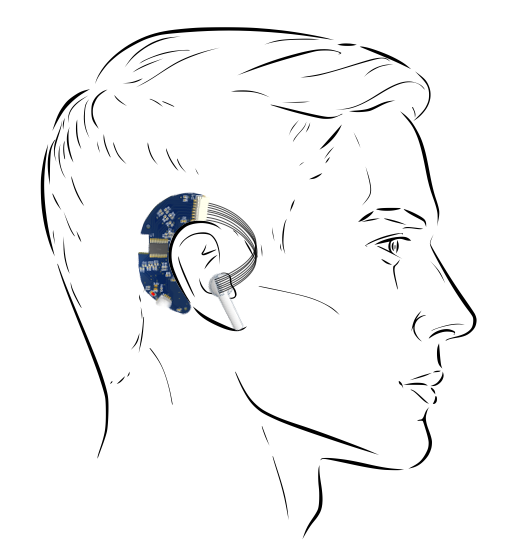
\includegraphics[width=0.48\textwidth]{thesis-doc/images/prototype/prototype_on_head_visual.png}
    \caption{Sketch and real view of the earpiece from different perspectives.
The sketch shows the first idea of how the FlexPCB has to be designed so that it gets through the earplug to the tip to measure in the direction of the tympanic membrane. The real views provide an impression of how the component is composed. Also can see the routing of the FlexPCB.}
    \label{fig:design:prototype_earpiece_views}
\end{figure}

\section{Study}
\label{ch:Design:Study}
This study aims to evaluate the accuracy of measuring core body temperature using an earable form factor device compared to a medical reference device.

Participants will be healthy adults. Demographic data like age, gender, weight, and size will be collected. Ear measurements like size and fit of the earbud sensors will also be noted.

Participants will first enter the room and sit still for 20 minutes to allow the sensors to calibrate and reach equilibrium \cite{chagllae.MeasurementCoreBody2018}. The room temperature will be fixed.

Data will be collected in three 10 minute phases:
\begin{enumerate}
\item Sitting
\item Walking outdoors
\item Sitting again
\end{enumerate}

Body temperature will be measured every 60 seconds using the earable device and a medical infrared tympanic thermometer for comparison \cite{chagllae.MeasurementCoreBody2018,boanoNoninvasiveMeasurementCore2013}.

\subsection{Data Analysis}
The accuracy of the earable device will be evaluated by comparing its temperature measurements to the medical reference device. Variability between different ear sensor positions will also be examined.

Environmental factors like ambient temperature, humidity, and subject motion will be analyzed for their impact on measurement accuracy and artifact reduction.